% Options for packages loaded elsewhere
\PassOptionsToPackage{unicode}{hyperref}
\PassOptionsToPackage{hyphens}{url}
\PassOptionsToPackage{dvipsnames,svgnames,x11names}{xcolor}
%
\documentclass[
  11pt,
]{article}
\usepackage{amsmath,amssymb}
\usepackage{iftex}
\ifPDFTeX
  \usepackage[T1]{fontenc}
  \usepackage[utf8]{inputenc}
  \usepackage{textcomp} % provide euro and other symbols
\else % if luatex or xetex
  \usepackage{unicode-math} % this also loads fontspec
  \defaultfontfeatures{Scale=MatchLowercase}
  \defaultfontfeatures[\rmfamily]{Ligatures=TeX,Scale=1}
\fi
\usepackage{lmodern}
\ifPDFTeX\else
  % xetex/luatex font selection
\fi
% Use upquote if available, for straight quotes in verbatim environments
\IfFileExists{upquote.sty}{\usepackage{upquote}}{}
\IfFileExists{microtype.sty}{% use microtype if available
  \usepackage[]{microtype}
  \UseMicrotypeSet[protrusion]{basicmath} % disable protrusion for tt fonts
}{}
\makeatletter
\@ifundefined{KOMAClassName}{% if non-KOMA class
  \IfFileExists{parskip.sty}{%
    \usepackage{parskip}
  }{% else
    \setlength{\parindent}{0pt}
    \setlength{\parskip}{6pt plus 2pt minus 1pt}}
}{% if KOMA class
  \KOMAoptions{parskip=half}}
\makeatother
\usepackage{xcolor}
\usepackage{microtype}
\usepackage[a4paper,margin=1in]{geometry}
\usepackage{color}
\usepackage{fancyvrb}
\newcommand{\VerbBar}{|}
\newcommand{\VERB}{\Verb[commandchars=\\\{\}]}
\DefineVerbatimEnvironment{Highlighting}{Verbatim}{commandchars=\\\{\},fontsize=\small}
% Add ',fontsize=\small' for more characters per line
\newenvironment{Shaded}{}{}
\newcommand{\AlertTok}[1]{\textcolor[rgb]{1.00,0.00,0.00}{\textbf{#1}}}
\newcommand{\AnnotationTok}[1]{\textcolor[rgb]{0.38,0.63,0.69}{\textbf{\textit{#1}}}}
\newcommand{\AttributeTok}[1]{\textcolor[rgb]{0.49,0.56,0.16}{#1}}
\newcommand{\BaseNTok}[1]{\textcolor[rgb]{0.25,0.63,0.44}{#1}}
\newcommand{\BuiltInTok}[1]{\textcolor[rgb]{0.00,0.50,0.00}{#1}}
\newcommand{\CharTok}[1]{\textcolor[rgb]{0.25,0.44,0.63}{#1}}
\newcommand{\CommentTok}[1]{\textcolor[rgb]{0.38,0.63,0.69}{\textit{#1}}}
\newcommand{\CommentVarTok}[1]{\textcolor[rgb]{0.38,0.63,0.69}{\textbf{\textit{#1}}}}
\newcommand{\ConstantTok}[1]{\textcolor[rgb]{0.53,0.00,0.00}{#1}}
\newcommand{\ControlFlowTok}[1]{\textcolor[rgb]{0.00,0.44,0.13}{\textbf{#1}}}
\newcommand{\DataTypeTok}[1]{\textcolor[rgb]{0.56,0.13,0.00}{#1}}
\newcommand{\DecValTok}[1]{\textcolor[rgb]{0.25,0.63,0.44}{#1}}
\newcommand{\DocumentationTok}[1]{\textcolor[rgb]{0.73,0.13,0.13}{\textit{#1}}}
\newcommand{\ErrorTok}[1]{\textcolor[rgb]{1.00,0.00,0.00}{\textbf{#1}}}
\newcommand{\ExtensionTok}[1]{#1}
\newcommand{\FloatTok}[1]{\textcolor[rgb]{0.25,0.63,0.44}{#1}}
\newcommand{\FunctionTok}[1]{\textcolor[rgb]{0.02,0.16,0.49}{#1}}
\newcommand{\ImportTok}[1]{\textcolor[rgb]{0.00,0.50,0.00}{\textbf{#1}}}
\newcommand{\InformationTok}[1]{\textcolor[rgb]{0.38,0.63,0.69}{\textbf{\textit{#1}}}}
\newcommand{\KeywordTok}[1]{\textcolor[rgb]{0.00,0.44,0.13}{\textbf{#1}}}
\newcommand{\NormalTok}[1]{#1}
\newcommand{\OperatorTok}[1]{\textcolor[rgb]{0.40,0.40,0.40}{#1}}
\newcommand{\OtherTok}[1]{\textcolor[rgb]{0.00,0.44,0.13}{#1}}
\newcommand{\PreprocessorTok}[1]{\textcolor[rgb]{0.74,0.48,0.00}{#1}}
\newcommand{\RegionMarkerTok}[1]{#1}
\newcommand{\SpecialCharTok}[1]{\textcolor[rgb]{0.25,0.44,0.63}{#1}}
\newcommand{\SpecialStringTok}[1]{\textcolor[rgb]{0.73,0.40,0.53}{#1}}
\newcommand{\StringTok}[1]{\textcolor[rgb]{0.25,0.44,0.63}{#1}}
\newcommand{\VariableTok}[1]{\textcolor[rgb]{0.10,0.09,0.49}{#1}}
\newcommand{\VerbatimStringTok}[1]{\textcolor[rgb]{0.25,0.44,0.63}{#1}}
\newcommand{\WarningTok}[1]{\textcolor[rgb]{0.38,0.63,0.69}{\textbf{\textit{#1}}}}
\usepackage{graphicx}
\usepackage{float}
\makeatletter
\def\maxwidth{\ifdim\Gin@nat@width>\linewidth\linewidth\else\Gin@nat@width\fi}
\def\maxheight{\ifdim\Gin@nat@height>\textheight\textheight\else\Gin@nat@height\fi}
\makeatother
% Scale images if necessary, so that they will not overflow the page
% margins by default, and it is still possible to overwrite the defaults
% using explicit options in \includegraphics[width, height, ...]{}
\setkeys{Gin}{width=\maxwidth,height=\maxheight,keepaspectratio}
% Set default figure placement to htbp
\makeatletter
\def\fps@figure{htbp}
\makeatother
\setlength{\emergencystretch}{8em} % prevent overfull lines
\providecommand{\tightlist}{%
  \setlength{\itemsep}{0pt}\setlength{\parskip}{0pt}}
\setcounter{secnumdepth}{-\maxdimen} % remove section numbering
\ifLuaTeX
\usepackage[bidi=basic]{babel}
\else
\usepackage[bidi=default]{babel}
\fi
\babelprovide[main,import]{spanish}
% get rid of language-specific shorthands (see #6817):
\let\LanguageShortHands\languageshorthands
\def\languageshorthands#1{}
\ifLuaTeX
  \usepackage{selnolig}  % disable illegal ligatures
\fi
\usepackage{bookmark}
\IfFileExists{xurl.sty}{\usepackage{xurl}}{} % add URL line breaks if available
\urlstyle{same}
\hypersetup{
  pdftitle={Extremizadores complete-split para un funcional fraccional de cobertura de triángulos en grafos cordales},
  pdflang={es-CL},
  colorlinks=true,
  linkcolor={blue},
  filecolor={Maroon},
  citecolor={Blue},
  urlcolor={Blue},
  pdfcreator={LaTeX via pandoc}}

\title{Extremizadores complete-split para un funcional fraccional de cobertura de triángulos en grafos cordales}
\author{Juan Pablo Traverso Gianini\\
\small Investigador independiente, Santiago, Chile\\
\small \href{mailto:jtraverso@gmail.com}{jtraverso@gmail.com}\\
\small ORCID: 0009-0003-6068-4096}
\date{10 de julio de 2026}

\begin{document}
\sloppy
\maketitle
\begin{small}\begin{raggedright}

\textbf{Paper II de la serie}\\
\textbf{Manuscrito preprint:} v1.0\\
\textbf{Fecha:} 10 de julio de 2026\\
\textbf{Estado:} lanzamiento de preprint; el teorema fraccional finito
exacto está probado analíticamente y verificado formalmente en Lean 4
con Mathlib v4.28.0 en el commit \texttt{5f2d448}; el desarrollo no
contiene \texttt{sorry} y su reporte de axiomas contiene solo los
axiomas fundacionales estándar de Lean (\texttt{propext},
\texttt{Classical.choice}, \texttt{Quot.sound}), sin axiomas específicos
del proyecto; no ha sido revisado externamente por pares; la revisión
bibliográfica y de novedad está incompleta \textbf{MSC 2020:} Primario
05C70; secundarios 05C35, 05C72.

\begin{center}\rule{0.5\linewidth}{0.5pt}\end{center}

\end{raggedright}\end{small}

\section{Resumen}\label{resumen}

Para un grafo \(G\), sea \(\tau_3^*(G)\) su número fraccional de
cobertura de triángulos, y definamos

\[
\Phi_\tau(G):=|E(G)|-2\tau_3^*(G).
\]

Determinamos el máximo exacto de \(\Phi_\tau\) sobre grafos cordales de
orden fijo. Para todo entero \(n\ge1\),

\[
\boxed{
\max_{\substack{|V(G)|=n\\G\text{ cordal}}}
\Phi_\tau(G)
=
\left\lfloor\frac{(2n+1)^2}{24}\right\rfloor.
}
\]

La prueba es finita y parte desde coberturas. Su paso principal es una
desigualdad de copia de vértices: para dos vértices no adyacentes, el
promedio de los valores de \(\Phi_\tau\) en las dos direcciones posibles
de copia es al menos el valor del grafo original. Un argumento de
convexidad discreta eleva este hecho desde vértices individuales a
clases completas de clones de vecindario abierto. En grafos cordales,
copiar hacia una clase de clones simplicial preserva la cordalidad. Las
copias admisibles repetidas reducen entonces el problema extremal, sin
disminuir \(\Phi_\tau\), a grafos complete-split

\[
S_{p,q}:=K_p\vee\overline{K_q}.
\]

En \(S_{p,q}\), el promedio por órbitas reduce el cálculo de la
cobertura fraccional a un programa lineal de dos variables. Resolver sus
dos ramas, incluido el caso degenerado \(S_{2,0}=K_2\), y luego
maximizar sobre \(p+q=n\), da exactamente la parte entera mostrada.

Este es el componente extremal fraccional finito del programa más amplio
sobre el Problema \#81 de Erdős. El artículo prueba solo el teorema
anterior para el funcional fraccional de cobertura. No prueba un teorema
integral de particiones en cliques, no usa dualidad fuerte de
programación lineal y no invoca un teorema asintótico de
empaquetamiento.

\textbf{Palabras clave:} grafo cordal; cobertura fraccional de
triángulos; simetrización; clase de clones; grafo complete-split;
problema de Erdős.

\begin{center}\rule{0.5\linewidth}{0.5pt}\end{center}

\section{1. Introducción}\label{introducciuxf3n}

Un grafo es cordal si no contiene ciclos inducidos de longitud al menos
cuatro. Los grafos cordales admiten varias descripciones estructurales
equivalentes, entre ellas órdenes de eliminación perfecta y árboles de
cliques. Estas descripciones hacen que la clase sea adecuada para
argumentos extremales en los que se simplifican vértices mientras se
controla un parámetro del grafo.

Este artículo estudia el funcional

\[
\Phi_\tau(G):=|E(G)|-2\tau_3^*(G),
\]

donde \(\tau_3^*(G)\) es el número fraccional de cobertura de
triángulos. El resultado principal es un teorema extremal finito exacto.

\subsubsection{Teorema 1.1}\label{teorema-1.1}

Para todo entero \(n\ge1\),

\[
\boxed{
\max_{\substack{|V(G)|=n\\G\text{ cordal}}}
\left(
|E(G)|-2\tau_3^*(G)
\right)
=
\left\lfloor\frac{(2n+1)^2}{24}\right\rfloor.
}
\]

Además, la igualdad se alcanza en un grafo complete-split

\[
S_{p,q}=K_p\vee\overline{K_q},
\qquad
p+q=n,
\]

con \(p\) entero más cercano a \((2n+1)/6\).

\subsubsection{Corolario 1.2}\label{corolario-1.2}

Para grafos cordales de orden \(n\),

\[
\max_{\substack{|V(G)|=n\\G\text{ cordal}}}\Phi_\tau(G)=\frac{n^2}{6}+O(n),
\]

de modo que el máximo es \((1+o(1))\,n^2/6\). La constante principal
\(1/6\) es la misma que aparece en el objetivo de
Erdős--Ordman--Zalcstein para particiones en cliques de grafos cordales
{[}1{]}. Esta afirmación se refiere solamente al funcional fraccional
\(\Phi_\tau\); aquí no se realiza el paso a una cota integral de
particiones en cliques.

\subsubsection{Prueba}\label{prueba}

Por el Teorema 1.1, el máximo es
\(\left\lfloor(2n+1)^2/24\right\rfloor\). Como
\((2n+1)^2/24=n^2/6+n/6+1/24\), la parte entera difiere de \(n^2/6+n/6\)
en menos de \(1\); por tanto, el máximo es \(n^2/6+O(n)\).

\textbf{Estado de verificación formal.} El Teorema 1.1 ha sido
verificado formalmente en Lean 4 con Mathlib v4.28.0 {[}5,6{]}, como
\texttt{PaperII.theorem\_1\_2} en el commit \texttt{5f2d448}. La
formalización es incondicional: su única hipótesis de cordalidad es la
definición estándar \texttt{IsChordal} --- todo ciclo de longitud al
menos cuatro tiene una cuerda. Los hechos estructurales de la Sección 2
--- cordalidad de subgrafos inducidos, preservación de cordalidad al
agregar un vértice con vecindario clique, y existencia de vértices
simpliciales --- se derivan de esa definición dentro del desarrollo, y
no se usa ningún axioma de árbol de cliques ni de intersección por
caminos. La caracterización terminal de la Sección 5 está formalizada
por un argumento sin árboles de cliques. La prueba no contiene
\texttt{sorry} y su huella axiomática es exactamente
\([\texttt{propext},\ \texttt{Classical.choice},\ \texttt{Quot.sound}]\),
los axiomas clásicos estándar de Lean, sin \texttt{sorryAx}. La Sección
8 registra los detalles.

La prueba tiene dos partes. La primera es estructural. Reduce un grafo
cordal arbitrario a un grafo complete-split sin disminuir \(\Phi_\tau\).
La segunda es un cálculo sobre esa familia terminal.

La idea estructural es la siguiente. Si \(u\) y \(v\) son no adyacentes,
el grafo \(G_{v\to u}\) se obtiene reemplazando el vecindario de \(v\)
por el vecindario de \(u\). Así \(v\) se convierte en un clon de \(u\).
Las dos operaciones opuestas de copia satisfacen

\[
\Phi_\tau(G_{v\to u})
+
\Phi_\tau(G_{u\to v})
\ge
2\Phi_\tau(G).
\]

Esta desigualdad es el paso básico de intercambio. Una cobertura óptima
de \(G\) se transporta a ambos grafos copiados. Los dos cambios en costo
de cobertura se cancelan al sumar las dos desigualdades. Los conteos de
aristas se cancelan del mismo modo.

Copiar un solo vértice no basta para una reducción terminante: puede
partir una clase de clones que ya existía. Por eso copiamos clases
completas de clones de vecindario abierto. La misma desigualdad de
intercambio se transforma en una afirmación de convexidad discreta para
una sucesión finita \(H_0,\ldots,H_{a+b}\). En consecuencia, una de las
dos direcciones de copia de clase completa no disminuye \(\Phi_\tau\).

Hay un punto en el que la cordalidad importa. La dirección no
decreciente la elige el argumento de convexidad, por lo que no se conoce
de antemano. Para mantener el grafo cordal cualquiera sea la dirección
elegida, las dos clases de clones se toman simpliciales. Copiar hacia
una clase simplicial es seguro porque los vértices copiados se
reinsertan con un vecindario que es clique.

La caracterización terminal se prueba por separado. A partir de la
propiedad de intersección por caminos de un árbol de cliques, un grafo
cordal en el que todo par de vértices simpliciales no adyacentes tiene
el mismo vecindario abierto debe ser complete-split. Por tanto, la
simetrización se detiene exactamente en la familia deseada.

En \(S_{p,q}\), el cálculo es breve, pero los casos pequeños deben
quedar visibles. El promedio por órbitas da un peso de cobertura \(x\)
en las aristas del clique y un peso \(y\) en las aristas radiales. Los
tipos posibles de triángulos producen

\[
3x\ge1
\quad(p\ge3),
\qquad
x+2y\ge1
\quad(p\ge2,\ q\ge1).
\]

Una restricción se incluye solo cuando existe el tipo de triángulo
correspondiente. En particular, \(S_{2,0}=K_2\) no tiene triángulos y su
número de cobertura es cero. Con esta convención, el programa lineal
terminal tiene dos ramas, y la maximización restante sobre \(p+q=n\) es
un cálculo entero de una variable.

\textbf{Relación con el Problema \#81 de Erdős.} Erdős, Ordman y
Zalcstein preguntaron por una cota superior de la forma \(n^2/6+O(n)\)
para particiones en cliques de grafos cordales {[}1{]}. El Teorema 1.1
identifica el extremo finito exacto del funcional fraccional de
cobertura que aparece en una ruta hacia ese problema. No pasa de
coberturas fraccionales a empaquetamientos integrales de triángulos ni a
particiones en cliques; esas interfaces pertenecen a trabajos separados.

Este es el segundo artículo de una serie. El Paper I estableció una cota
fraccional finita, \(|E(G)|-2\nu_3^*(G)\le n^2/6+n\), para grafos split;
el presente artículo determina el máximo fraccional exacto sobre todos
los grafos cordales. El paso restante desde este funcional fraccional a
una cota integral de particiones en cliques --- la interfaz con el
Problema \#81 de Erdős propiamente tal --- no se trata aquí.

La Sección 2 fija la notación y los hechos cordales usados después. Las
Secciones 3 y 4 prueban la desigualdad de copia y su forma para clases
de clones. La Sección 5 da la caracterización terminal y la reducción a
grafos complete-split. Las Secciones 6 y 7 resuelven el programa
terminal y ensamblan el teorema. La Sección 8 registra reproducibilidad,
alcance de la verificación formal y estado de validación.

\begin{center}\rule{0.5\linewidth}{0.5pt}\end{center}

\section{2. Definiciones y preliminares
cordales}\label{definiciones-y-preliminares-cordales}

Todos los grafos son finitos y simples. Escribimos \(V(G)\), \(E(G)\), y

\[
e(G):=|E(G)|.
\]

Sea \(\mathcal T(G)\) el conjunto de triángulos de \(G\).

Una \textbf{cobertura fraccional de triángulos} es una función

\[
z:E(G)\longrightarrow\mathbb R_{\ge0}
\]

tal que

\[
\sum_{e\in E(T)}z_e\ge1
\qquad (T\in\mathcal T(G)).
\]

Su costo es \(\sum_{e\in E(G)}z_e\), y

\[
\tau_3^*(G)
:=
\min\left\{
\sum_{e\in E(G)}z_e:
z\text{ es una cobertura fraccional de triángulos}
\right\}.
\]

El mínimo se alcanza porque este es un programa lineal finito factible y
acotado inferiormente por cero. Si \(G\) no tiene triángulos, entonces
\(\tau_3^*(G)=0\).

Definimos

\[
\Phi_\tau(G):=e(G)-2\tau_3^*(G).
\]

Para \(p,q\ge0\), el \textbf{grafo complete-split}

\[
S_{p,q}:=K_p\vee\overline{K_q}
\]

tiene un lado clique \(K\) de orden \(p\), un lado independiente \(I\)
de orden \(q\), y todas las \(pq\) aristas entre ambos lados.

Dos vértices \(u,v\) son \textbf{clones de vecindario abierto} si

\[
N_G(u)=N_G(v).
\]

Clones distintos de vecindario abierto son necesariamente no adyacentes.
Una clase de clones es un conjunto maximal de vértices que son clones
dos a dos. Sea \(m(G)\) el número de clases maximales de clones.

Un vértice \(v\) es \textbf{simplicial} si \(N_G(v)\) es un clique. Una
clase de clones es simplicial si su vecindario abierto común es un
clique.

Para vértices no adyacentes \(u,v\), sea \(G_{v\to u}\) el grafo
obtenido eliminando todas las aristas incidentes con \(v\) y luego
uniendo \(v\) a todos los vértices de \(N_G(u)\). Así, \(u\) y \(v\) son
clones en \(G_{v\to u}\).

Usamos los siguientes hechos estándar sobre grafos cordales {[}2,3{]}.

\begin{enumerate}
\def\labelenumi{\arabic{enumi}.}
\tightlist
\item
  Todo subgrafo inducido de un grafo cordal es cordal.
\item
  Agregar un nuevo vértice cuyo vecindario es un clique preserva la
  cordalidad.
\item
  Todo grafo cordal no vacío tiene un vértice simplicial, y todo grafo
  cordal conexo no completo tiene dos vértices simpliciales no
  adyacentes.
\item
  Todo grafo cordal conexo tiene un árbol de cliques: sus nodos son los
  cliques maximales, y los cliques maximales que contienen un vértice
  fijo inducen un subárbol conexo.
\end{enumerate}

También usamos dos hechos elementales sobre árboles: un árbol con al
menos dos nodos tiene al menos dos hojas, y un subárbol conexo que
contiene todas las hojas es el árbol completo.

\begin{center}\rule{0.5\linewidth}{0.5pt}\end{center}

\section{3. La desigualdad de copia de
vértices}\label{la-desigualdad-de-copia-de-vuxe9rtices}

\subsubsection{Lema 3.1}\label{lema-3.1}

Sea \(G\) un grafo y sean \(u,v\in V(G)\) no adyacentes. Entonces

\[
\boxed{
\Phi_\tau(G_{v\to u})
+
\Phi_\tau(G_{u\to v})
\ge
2\Phi_\tau(G).
}
\]

\subsubsection{Prueba}\label{prueba-1}

Sea \(z\) una cobertura fraccional óptima de triángulos de \(G\), de
modo que

\[
\sum_{e\in E(G)}z_e=\tau_3^*(G).
\]

Primero construimos una cobertura \(z'\) de \(G_{v\to u}\). Para una
arista no incidente con \(v\), conservamos su peso anterior. Para cada
\(x\in N_G(u)\), ponemos

\[
z'_{vx}:=z_{ux}.
\]

Para verificar factibilidad, consideremos un triángulo de
\(G_{v\to u}\). Si no contiene \(v\), entonces es un triángulo de \(G\)
y los tres pesos no cambian. Si es \(vxy\), entonces \(x,y\in N_G(u)\) y
\(xy\in E(G)\). Por tanto, \(uxy\) es un triángulo de \(G\), y

\[
z'_{vx}+z'_{vy}+z'_{xy}
=
z_{ux}+z_{uy}+z_{xy}
\ge1.
\]

Así, \(z'\) es factible.

Su costo es

\[
\operatorname{cost}(z')
=
\left(
\sum_{e\in E(G)}z_e
-
\sum_{x\in N_G(v)}z_{vx}
\right)
+
\sum_{x\in N_G(u)}z_{ux}.
\tag{3.1}
\]

Intercambiando \(u\) y \(v\), obtenemos una cobertura factible \(z''\)
de \(G_{u\to v}\) con

\[
\operatorname{cost}(z'')
=
\left(
\sum_{e\in E(G)}z_e
-
\sum_{x\in N_G(u)}z_{ux}
\right)
+
\sum_{x\in N_G(v)}z_{vx}.
\tag{3.2}
\]

Al sumar (3.1) y (3.2), los términos de corrección se cancelan
exactamente:

\[
\operatorname{cost}(z')
+
\operatorname{cost}(z'')
=
2\tau_3^*(G).
\]

Como cada óptimo es no mayor que el costo de la cobertura factible
correspondiente,

\[
\tau_3^*(G_{v\to u})
+
\tau_3^*(G_{u\to v})
\le
2\tau_3^*(G).
\tag{3.3}
\]

Los conteos de aristas satisfacen una segunda identidad exacta. El grafo
\(G_{v\to u}\) reemplaza \(d_G(v)\) por \(d_G(u)\) y no cambia ninguna
arista no incidente con \(v\). Por tanto,

\[
e(G_{v\to u})
=
e(G)-d_G(v)+d_G(u).
\]

Análogamente,

\[
e(G_{u\to v})
=
e(G)-d_G(u)+d_G(v).
\]

Luego

\[
e(G_{v\to u})+e(G_{u\to v})=2e(G).
\tag{3.4}
\]

Usando la definición de \(\Phi_\tau\), restamos dos veces (3.3) a (3.4):

\[
\begin{aligned}
\Phi_\tau(G_{v\to u})
+
\Phi_\tau(G_{u\to v})
&=
2e(G)
-
2\left(
\tau_3^*(G_{v\to u})
+
\tau_3^*(G_{u\to v})
\right)\\
&\ge
2e(G)-4\tau_3^*(G)\\
&=
2\Phi_\tau(G).
\end{aligned}
\]

Esto prueba el lema.

\subsubsection{Corolario 3.2}\label{corolario-3.2}

Al menos uno de los dos grafos \(G_{v\to u}\) y \(G_{u\to v}\) satisface

\[
\Phi_\tau(G_{\mathrm{copy}})\ge\Phi_\tau(G).
\]

No se necesita ninguna normalización del tipo \(z_e\le1\) en la prueba.

\begin{center}\rule{0.5\linewidth}{0.5pt}\end{center}

\section{4. Copia de clases completas de
clones}\label{copia-de-clases-completas-de-clones}

Sean \(U,V\) clases de clones distintas y no adyacentes, con

\[
|U|=a,
\qquad
|V|=b.
\]

Fuera de \(U\cup V\), mantenemos fijo el grafo. Para \(0\le k\le a+b\),
sea \(H_k\) el grafo en el que \(k\) vértices de \(U\cup V\) tienen tipo
de vecindario \(N(U)\), y los \(a+b-k\) restantes tienen tipo de
vecindario \(N(V)\). Todos los vértices de \(U\cup V\) siguen siendo no
adyacentes entre sí. Salvo isomorfismo,

\[
H_a=G,
\qquad
H_0=G_{U\to V},
\qquad
H_{a+b}=G_{V\to U}.
\]

\subsubsection{Lema 4.1}\label{lema-4.1}

Para

\[
f(k):=\Phi_\tau(H_k),
\]

se tiene

\[
f(k-1)+f(k+1)\ge2f(k)
\qquad
(1\le k\le a+b-1).
\]

En consecuencia,

\[
f(a)\le\max\{f(0),f(a+b)\}.
\]

\subsubsection{Prueba}\label{prueba-2}

Sea \(k\) con \(1\le k\le a+b-1\). Entonces \(H_k\) contiene al menos un
vértice \(x\) de tipo \(U\) y un vértice \(y\) de tipo \(V\). Estos dos
vértices no son adyacentes. En \(H_k\), copiar \(x\) hacia \(y\) cambia
un vértice de tipo \(U\) en un vértice de tipo \(V\), por lo que el
grafo resultante es isomorfo a \(H_{k-1}\). Copiar \(y\) hacia \(x\) da
un grafo isomorfo a \(H_{k+1}\). El Lema 3.1 da entonces

\[
f(k-1)+f(k+1)\ge2f(k).
\]

Pongamos

\[
\Delta_k:=f(k)-f(k-1).
\]

La desigualdad anterior equivale a

\[
\Delta_{k+1}\ge\Delta_k.
\]

Así, las primeras diferencias son no decrecientes. Una sucesión finita
de este tipo no puede tener un máximo estricto en el interior: antes de
que las diferencias se vuelvan no negativas, la sucesión decrece;
después de ese punto, no decrece. Por tanto, el máximo de
\(f(0),\ldots,f(a+b)\) se alcanza en un extremo, y en particular

\[
f(a)\le\max\{f(0),f(a+b)\}.
\]

Esto dice exactamente que una de las dos direcciones de copia de clase
completa no disminuye \(\Phi_\tau\).

\subsubsection{Lema 4.2}\label{lema-4.2}

Después de copiar una clase completa de clones sobre otra, ninguna clase
antigua de clones se parte. La clase fuente y la clase objetivo se
fusionan, y por tanto el número de clases maximales de clones decrece
estrictamente.

\subsubsection{Prueba}\label{prueba-3}

Supongamos que la clase fuente \(W_1\) se copia sobre la clase objetivo
\(W_2\), cuyo vecindario común es \(B\). Todo vértice de \(W_1\cup W_2\)
tiene vecindario \(B\) en el grafo nuevo, por lo que estas dos clases se
fusionan.

Sea \(C\) una clase antigua de clones disjunta de \(W_1\cup W_2\), y
sean \(c,c'\in C\). Las aristas no incidentes con \(W_1\) no cambian, de
modo que \(c\) y \(c'\) siguen coincidiendo en todas las coordenadas
fuera de \(W_1\). Para \(w\in W_1\), la adyacencia a \(w\) en el grafo
nuevo equivale a pertenecer a \(B\). Como \(B=N_G(W_2)\) y \(c,c'\) eran
clones en \(G\), ambos pertenecen a \(B\) o ninguno pertenece a \(B\).
Por tanto, \(c,c'\) también coinciden en todas las coordenadas dentro de
\(W_1\). Luego \(C\) no se parte.

Las dos clases distintas \(W_1,W_2\) se fusionan y toda otra clase
antigua queda contenida en una clase nueva. Por consiguiente, las clases
antiguas se proyectan sobre las nuevas, con dos clases antiguas
identificadas y ninguna partida. Luego \(m(G)\) decrece estrictamente.

\subsubsection{Lema 4.3}\label{lema-4.3}

Si \(G\) es cordal y la clase de clones objetivo es simplicial, entonces
copiar sobre ella una clase de clones no adyacente preserva la
cordalidad.

\subsubsection{Prueba}\label{prueba-4}

Eliminamos la clase fuente. El grafo restante es un subgrafo inducido de
\(G\), por tanto es cordal. Reinsertamos los vértices de la clase fuente
uno por uno, cada uno con el vecindario común de la clase objetivo. Ese
vecindario es un clique porque la clase objetivo es simplicial. Agregar
un vértice con vecindario clique preserva la cordalidad.

La dirección entregada por el Lema 4.1 no se conoce de antemano. Por
esta razón, la simetrización usará pares en los que ambas clases son
simpliciales.

\begin{center}\rule{0.5\linewidth}{0.5pt}\end{center}

\section{5. Grafos cordales terminales y
simetrización}\label{grafos-cordales-terminales-y-simetrizaciuxf3n}

Primero caracterizamos los grafos terminales sin referencia al proceso
de copia.

\subsubsection{Lema 5.1}\label{lema-5.1}

Sea \(H\) un grafo cordal finito con la siguiente propiedad:

\begin{quote}
todo par de vértices simpliciales no adyacentes de \(H\) tiene el mismo
vecindario abierto.
\end{quote}

Entonces \(H\) es complete-split.

\emph{La formalización Lean acompañante prueba este lema mediante un
argumento equivalente que no usa árboles de cliques --- usando
eliminación simplicial y el hecho de que todo separador minimal de
vértices de un grafo cordal es un clique --- en lugar de la prueba con
árbol de cliques dada abajo; véase §8. El enunciado probado es
idéntico.}

\subsubsection{Prueba}\label{prueba-5}

Si \(|V(H)|\le1\), la conclusión es inmediata. Supongamos primero que
\(H\) es disconexo. Si una componente contiene una arista y otra
componente es no vacía, elegimos un vértice simplicial \(z\) con un
vecino en la primera componente y un vértice simplicial \(w\) en la otra
componente. Tales vértices existen por el teorema estándar de vértices
simpliciales aplicado dentro de cada componente. Son no adyacentes. La
hipótesis da

\[
N_H(z)=N_H(w).
\]

Los dos vecindarios viven en componentes distintas, por lo que ambos
tendrían que ser vacíos, contradiciendo que \(z\) tiene un vecino. Por
tanto, un \(H\) disconexo que satisface la hipótesis es edgeless, y así
es \(S_{0,|V(H)|}\).

Si \(H\) es completo, es \(S_{|V(H)|,0}\). Podemos suponer entonces que
\(H\) es conexo y no completo.

Elegimos un árbol de cliques \(\mathcal Q\) de \(H\). Tiene al menos dos
nodos y, por tanto, al menos dos hojas. Todo clique maximal hoja \(L\)
tiene un vértice privado, es decir, un vértice que no pertenece a ningún
otro clique maximal. En efecto, de lo contrario \(L\) estaría contenido
en la unión del clique vecino a lo largo de la única arista del árbol
que sale de \(L\), contradiciendo su maximalidad. Un vértice privado
\(x\) es simplicial, y su vecindario abierto es \(L\backslash\{x\}\).

Los vértices privados pertenecientes a cliques hoja distintos son no
adyacentes. En efecto, si \(x\in L_1\) y \(y\in L_2\), con
\(L_1\ne L_2\), fueran adyacentes, entonces algún clique maximal
contendría a ambos. Como \(x\) pertenece solo a \(L_1\), ese clique
tendría que ser \(L_1\), forzando \(y\in L_1\), en contradicción con la
privacidad de \(y\) en \(L_2\).

Por la hipótesis, todos los vértices privados de hojas tienen un
vecindario abierto común; llamémoslo \(K\). Por tanto, cada clique hoja
tiene la forma

\[
L=K\cup\{x_L\}.
\]

No puede haber dos vértices privados en un mismo clique hoja. Dos
vértices así serían adyacentes, y cada uno pertenecería al vecindario
común \(K\) de un vértice privado de otra hoja, contradiciendo la no
adyacencia recién probada.

Mostramos ahora que todo vértice de \(K\) es universal. Fijemos
\(v\in K\). Como \(v\) está en cada clique hoja, el subárbol conexo de
cliques maximales que contienen \(v\) contiene todas las hojas de
\(\mathcal Q\). Un subárbol conexo que contiene todas las hojas es todo
el árbol. Así, \(v\) pertenece a cada clique maximal y es adyacente a
todos los demás vértices de \(H\). Por tanto, \(K\) es un clique de
vértices universales.

Resta probar que \(H-K\) es independiente. Supongamos que \(H-K\)
contiene una arista. Una componente no trivial de \(H-K\) es cordal y
tiene un vértice simplicial \(z\) con un vecino dentro de esa
componente. Como cada vértice de \(K\) es universal,

\[
N_H(z)=K\cup N_{H-K}(z).
\]

Ambos conjuntos del lado derecho son cliques, y todas las aristas entre
ellos están presentes. Así \(z\) es simplicial en \(H\), y

\[
N_H(z)\supsetneq K.
\]

Elegimos un vértice privado de hoja \(x\), de modo que \(N_H(x)=K\).
Como \(z\notin K\), los vértices \(z\) y \(x\) no son adyacentes. La
hipótesis forzaría \(N_H(z)=N_H(x)=K\), una contradicción.

Por tanto, \(H-K\) es independiente. Como \(K\) es un clique universal,

\[
H=K_{|K|}\vee\overline{K_{|H-K|}},
\]

que es complete-split.

\subsubsection{Corolario 5.2}\label{corolario-5.2}

Si un grafo cordal no es complete-split, entonces tiene dos vértices
simpliciales no adyacentes con vecindarios abiertos distintos. Sus
clases de clones son distintas, no adyacentes y ambas simpliciales.

\subsubsection{Prueba}\label{prueba-6}

La primera afirmación es la contrapositiva del Lema 5.1. Sean \(x,y\)
los vértices resultantes y sean \(U,V\) sus clases de clones. Las clases
son simpliciales porque sus vecindarios comunes son \(N(x)\) y \(N(y)\),
ambos cliques. Son distintas porque esos vecindarios difieren.

Son no adyacentes como clases. Si algún \(u\in U\) y algún \(v\in V\)
fueran adyacentes, entonces \(v\in N(u)=N(x)\), y por simetría de la
adyacencia \(x\in N(v)=N(y)\). Esto haría adyacentes a \(x\) e \(y\), en
contradicción con su elección.

\subsubsection{Teorema 5.3}\label{teorema-5.3}

Para todo grafo cordal \(G\) con \(n\) vértices, existen enteros
\(p,q\ge0\), con \(p+q=n\), tales que

\[
\boxed{
\Phi_\tau(G)\le\Phi_\tau(S_{p,q}).
}
\]

\subsubsection{Prueba}\label{prueba-7}

Partiendo de \(G\), repetimos la siguiente operación mientras el grafo
actual no sea complete-split.

Por el Corolario 5.2, elegimos dos clases de clones simpliciales,
distintas y no adyacentes, con vecindarios distintos. Por el Lema 4.1,
una de las dos direcciones de copia de clase completa no disminuye
\(\Phi_\tau\). Ambos objetivos posibles son simpliciales, de modo que el
Lema 4.3 preserva la cordalidad cualquiera sea la dirección
seleccionada. Por el Lema 4.2, el número de clases maximales de clones
decrece estrictamente.

El proceso termina porque \(m(G)\) es un entero positivo. Al terminar no
queda ningún par dado por el Corolario 5.2, y por tanto el grafo es
complete-split por el Lema 5.1. Copiar nunca cambia el conjunto de
vértices, de modo que el grafo terminal es \(S_{p,q}\) con \(p+q=n\).
Como \(\Phi_\tau\) nunca disminuye,

\[
\Phi_\tau(G)\le\Phi_\tau(S_{p,q}).
\]

El requisito de que ambas clases sean simpliciales se usa solo para
hacer compatible este último argumento con la dirección escogida por
convexidad discreta.

\begin{center}\rule{0.5\linewidth}{0.5pt}\end{center}

\section{6. El programa de cobertura en
complete-split}\label{el-programa-de-cobertura-en-complete-split}

Sea

\[
S_{p,q}=K_p\vee\overline{K_q},
\qquad
P:=\binom p2.
\]

El grupo de automorfismos es

\[
\operatorname{Aut}(S_{p,q})
\cong
\mathfrak S_p\times\mathfrak S_q.
\]

Tiene dos órbitas de aristas: las \(P\) aristas del clique y las \(pq\)
aristas radiales.

\begin{figure}[H]
\centering
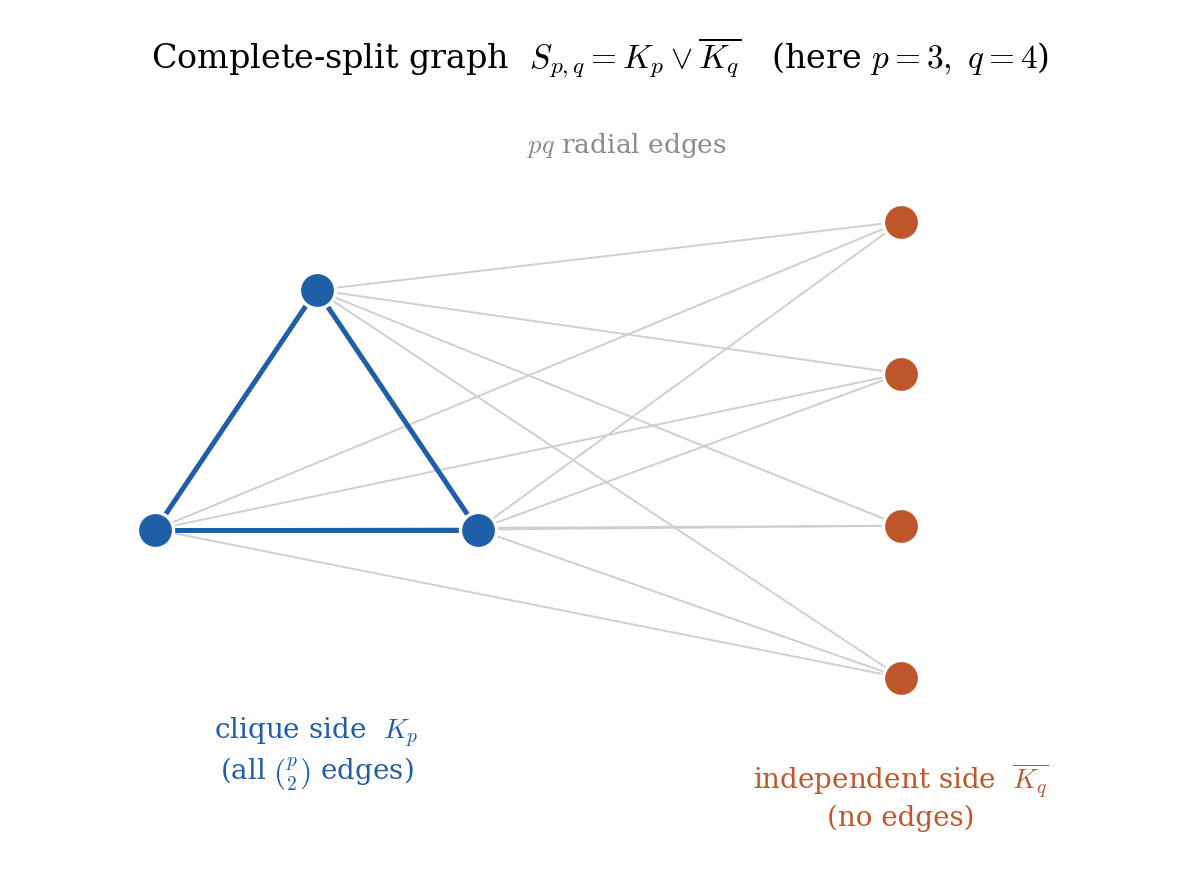
\includegraphics[width=0.45\textwidth,height=\textheight]{figures/fig1_completesplit.png}
\caption{El grafo complete-split \(S_{p,q}=K_p\vee\overline{K_q}\),
mostrado para \(p=3\), \(q=4\): un lado clique \(K_p\) con todas las
\(\binom p2\) aristas, un lado independiente \(\overline{K_q}\) sin
aristas internas, y todas las \(pq\) aristas radiales entre ambos lados.
El grupo de automorfismos \(\mathfrak S_p\times\mathfrak S_q\) tiene
exactamente estas dos órbitas de aristas, lo que hace posible la
reducción por promedio de órbitas del Lema 6.1.}
\end{figure}

\subsubsection{Lema 6.1}\label{lema-6.1}

Existe una cobertura fraccional óptima de triángulos de \(S_{p,q}\) que
es constante en cada órbita de aristas.

\subsubsection{Prueba}\label{prueba-8}

Sea \(z\) una cobertura óptima. Para cada automorfismo \(\sigma\),
transportamos \(z\) poniendo

\[
z^\sigma_e:=z_{\sigma^{-1}(e)}.
\]

Los automorfismos permutan triángulos, por lo que cada \(z^\sigma\) es
factible. Todos tienen el mismo costo. Su promedio

\[
\overline z
=
\frac{1}{|\operatorname{Aut}(S_{p,q})|}
\sum_{\sigma\in\operatorname{Aut}(S_{p,q})}z^\sigma
\]

es factible por convexidad, tiene el mismo costo, y es invariante bajo
el grupo de automorfismos. Por tanto, es constante en cada órbita de
aristas.

Escribimos \(x\) para el peso común en las aristas del clique y \(y\)
para el peso común en las aristas radiales. Hay dos tipos posibles de
triángulos.

\begin{itemize}
\tightlist
\item
  Tres vértices del clique, presentes solo cuando \(p\ge3\), dan \[
  3x\ge1.
  \]
\item
  Dos vértices del clique y un vértice independiente, presentes solo
  cuando \(p\ge2\) y \(q\ge1\), dan \[
  x+2y\ge1.
  \]
\end{itemize}

Así, el programa simetrizado es

\[
\min\{Px+pq\,y:x,y\ge0\},
\]

con cada restricción incluida solo cuando existe su tipo de triángulo.

\subsubsection{Proposición 6.2}\label{proposiciuxf3n-6.2}

Los casos degenerados son

\[
\tau_3^*(S_{p,q})=0
\qquad
(p\le1),
\]

y

\[
\tau_3^*(S_{2,0})=0.
\]

En todos los demás casos,

\[
\boxed{
\tau_3^*(S_{p,q})
=
\begin{cases}
\dfrac{P+pq}{3},
& p\ge3,\ 0\le q\le p-1,\\[3mm]
P,
& p\ge2,\ q\ge p-1.
\end{cases}
}
\]

\subsubsection{Prueba}\label{prueba-9}

Si \(p\le1\), el grafo no tiene triángulos. Lo mismo ocurre para
\(S_{2,0}=K_2\). Por tanto, el número de cobertura es cero en estos
casos.

Sea \(p\ge3\) y \(q=0\). Solo existe la restricción \(3x\ge1\), así que

\[
\tau_3^*(S_{p,0})
=
\min\{Px:3x\ge1,\ x\ge0\}
=
\frac P3.
\]

Esta es la primera rama con \(q=0\).

Ahora sea \(p\ge3\) y \(q\ge1\). Existen ambas restricciones. La
factibilidad fuerza \(x\ge1/3\). Si \(x>1\), bajar \(x\) a \(1\) y
mantener \(y=0\) no puede aumentar el objetivo, por lo que basta
considerar \(1/3\le x\le1\). Para tal \(x\), el menor valor factible de
\(y\) es

\[
y=\frac{1-x}{2}.
\]

Usar un \(y\) mayor solo aumenta el objetivo. Por tanto, el objetivo se
reduce a

\[
\begin{aligned}
Px+pq\,y
&=
Px+pq\frac{1-x}{2}\\
&=
\frac{pq}{2}
+
x\left(P-\frac{pq}{2}\right),
\end{aligned}
\]

y

\[
P-\frac{pq}{2}
=
\frac p2(p-1-q).
\]

Si \(q\le p-1\), este coeficiente es no negativo. El mínimo ocurre en
\(x=1/3\), y entonces \(y=1/3\). Su valor es

\[
\frac{P+pq}{3}.
\]

Si \(q\ge p-1\), el coeficiente es no positivo. El mínimo ocurre en
\(x=1\), \(y=0\), con valor \(P\).

Finalmente, supongamos \(p=2\) y \(q\ge1\). No hay triángulos
completamente dentro del clique, por lo que \(3x\ge1\) está ausente.
Como \(P=1\), el programa es

\[
\min\{x+2q\,y:x,y\ge0,\ x+2y\ge1\}.
\]

Para \(q\ge1\), el mínimo se alcanza en \(x=1\), \(y=0\), y vale
\(1=P\).

Cuando \(p\ge3\) y \(q=p-1\), las dos fórmulas coinciden porque

\[
\frac{P+p(p-1)}{3}=P.
\]

\subsubsection{Corolario 6.3}\label{corolario-6.3}

Para \(p+q=n\), el valor de \(\Phi_\tau(S_{p,q})\) es el siguiente.

En la rama \(q\ge p-1\),

\[
\Phi_\tau(S_{p,q})
=
pq-P
=
\frac{p(2n+1-3p)}2.
\tag{6.1}
\]

En la rama \(q\le p-1\), con \(p\ge3\),

\[
\Phi_\tau(S_{p,q})
=
\frac{P+pq}{3}
=
\frac{p(2n-p-1)}6.
\tag{6.2}
\]

Los casos degenerados se obtienen directamente de \(\tau_3^*=0\).

\subsubsection{Prueba}\label{prueba-10}

En la primera rama, la Proposición 6.2 da \(\tau_3^*=P\). Por tanto,

\[
\begin{aligned}
\Phi_\tau(S_{p,q})
&=
P+pq-2P\\
&=
pq-P\\
&=
p(n-p)-\frac{p(p-1)}2\\
&=
\frac{p(2n+1-3p)}2.
\end{aligned}
\]

En la segunda rama,

\[
\begin{aligned}
\Phi_\tau(S_{p,q})
&=
P+pq-\frac23(P+pq)\\
&=
\frac{P+pq}{3}\\
&=
\frac{p(p-1)+2p(n-p)}6\\
&=
\frac{p(2n-p-1)}6.
\end{aligned}
\]

\begin{center}\rule{0.5\linewidth}{0.5pt}\end{center}

\section{7. Maximización entera
exacta}\label{maximizaciuxf3n-entera-exacta}

\subsubsection{Proposición 7.1}\label{proposiciuxf3n-7.1}

Para enteros \(p,q\ge0\) con \(p+q=n\),

\[
\Phi_\tau(S_{p,q})
\le
\left\lfloor\frac{(2n+1)^2}{24}\right\rfloor.
\]

La igualdad se alcanza en la rama \(q\ge p-1\) con un entero \(p\) más
cercano a \((2n+1)/6\).

\subsubsection{Prueba}\label{prueba-11}

Primero consideramos la rama \(q\ge p-1\). Por (6.1),

\[
F_n(p)
:=
\Phi_\tau(S_{p,q})
=
\frac{p(2n+1-3p)}2.
\]

Completando el cuadrado,

\[
F_n(p)
=
\frac{(2n+1)^2}{24}
-
\frac32
\left(
p-\frac{2n+1}{6}
\right)^2.
\tag{7.1}
\]

Como \(F_n(p)\) es entero para \(p\) entero,

\[
F_n(p)
\le
\left\lfloor\frac{(2n+1)^2}{24}\right\rfloor.
\]

Queda mostrar que se alcanza la parte entera. Escribimos

\[
2n+1=6k+r,
\qquad
r\in\{1,3,5\}.
\]

Si \(r=1\), tomamos \(p=k\). La distancia cuadrada en (7.1) es \(1/36\),
y

\[
F_n(k)
=
\frac{(2n+1)^2-1}{24}.
\]

Si \(r=3\), tomamos \(p=k\) o \(p=k+1\). La distancia cuadrada es
\(1/4\), y

\[
F_n(p)
=
\frac{(2n+1)^2-9}{24}.
\]

Si \(r=5\), tomamos \(p=k+1\). Nuevamente la distancia cuadrada es
\(1/36\), y

\[
F_n(k+1)
=
\frac{(2n+1)^2-1}{24}.
\]

Un cuadrado impar es congruente con \(1\pmod{24}\), salvo que sea
divisible por \(3\), en cuyo caso es congruente con \(9\pmod{24}\). Por
tanto, cada valor mostrado es exactamente

\[
\left\lfloor\frac{(2n+1)^2}{24}\right\rfloor.
\]

El \(p\) elegido es más cercano a \((2n+1)/6\) y satisface

\[
p\le\frac{n+1}{2},
\]

lo cual equivale a \(q\ge p-1\). Por tanto, pertenece a la rama
considerada.

Ahora consideramos la rama \(q\le p-1\). Entonces

\[
p\ge\frac{n+1}{2},
\]

y (6.2) da

\[
\Phi_\tau(S_{p,q})
=
\frac{p(2n-p-1)}6.
\]

El numerador es una cuadrática cóncava en \(p\), con vértice real en
\(p=n-\tfrac12\). En el intervalo entero

\[
\left\lceil\frac{n+1}{2}\right\rceil
\le p\le n,
\]

el vértice queda entre los dos enteros más grandes, \(n-1\) y \(n\). Por
tanto, el máximo en este intervalo se alcanza en uno de esos dos puntos,
y ambos dan \(n(n-1)\). Luego

\[
\Phi_\tau(S_{p,q})
\le
\frac{n(n-1)}6.
\]

Para \(n\ge3\),

\[
\begin{aligned}
\frac{(2n+1)^2}{24}
-
\frac{n(n-1)}6
&=
\frac{(2n+1)^2-4n(n-1)}{24}\\
&=
\frac{8n+1}{24}\\
&>1.
\end{aligned}
\]

En consecuencia,

\[
\frac{n(n-1)}6
\le
\left\lfloor\frac{(2n+1)^2}{24}\right\rfloor.
\]

Los casos \(n\le2\), incluido \(S_{2,0}\), se verifican por inspección.
Así, la rama no saturada nunca excede el valor alcanzado en la rama
saturada.

\subsubsection{Prueba del Teorema 1.1}\label{prueba-del-teorema-1.1}

Sea \(G\) un grafo cordal con \(n\) vértices. El Teorema 5.3 da
\(p,q\ge0\), con \(p+q=n\), tales que

\[
\Phi_\tau(G)\le\Phi_\tau(S_{p,q}).
\]

La Proposición 7.1 da entonces

\[
\Phi_\tau(G)
\le
\left\lfloor\frac{(2n+1)^2}{24}\right\rfloor.
\]

Esto prueba la cota superior.

Para la igualdad, elegimos un entero \(p\) más cercano a \((2n+1)/6\), y
ponemos \(q=n-p\). Como en la Proposición 7.1, esta elección satisface
\(q\ge p-1\), por lo que pertenece a la rama saturada. La Proposición
7.1 da

\[
\Phi_\tau(S_{p,q})
=
\left\lfloor\frac{(2n+1)^2}{24}\right\rfloor.
\]

El grafo \(S_{p,q}\) es cordal, de modo que es admisible en el máximo.
Por lo tanto,

\[
\max_{\substack{|V(G)|=n\\G\text{ cordal}}}
\Phi_\tau(G)
=
\left\lfloor\frac{(2n+1)^2}{24}\right\rfloor.
\]

Esto completa la prueba.

\subsection{Ilustración numérica y casos
pequeños}\label{ilustraciuxf3n-numuxe9rica-y-casos-pequeuxf1os}

La siguiente figura muestra el caso \(n=12\). La rama saturada alcanza
su máximo en \(p=4\), \(q=8\), con valor

\[
\Phi_\tau(S_{4,8})=26
=
\left\lfloor\frac{25^2}{24}\right\rfloor.
\]

La línea punteada vertical marca el vértice real \(p=(2n+1)/6\), y la
línea vertical de cambio de rama marca \(p=(n+1)/2\).

\begin{figure}[H]
\centering
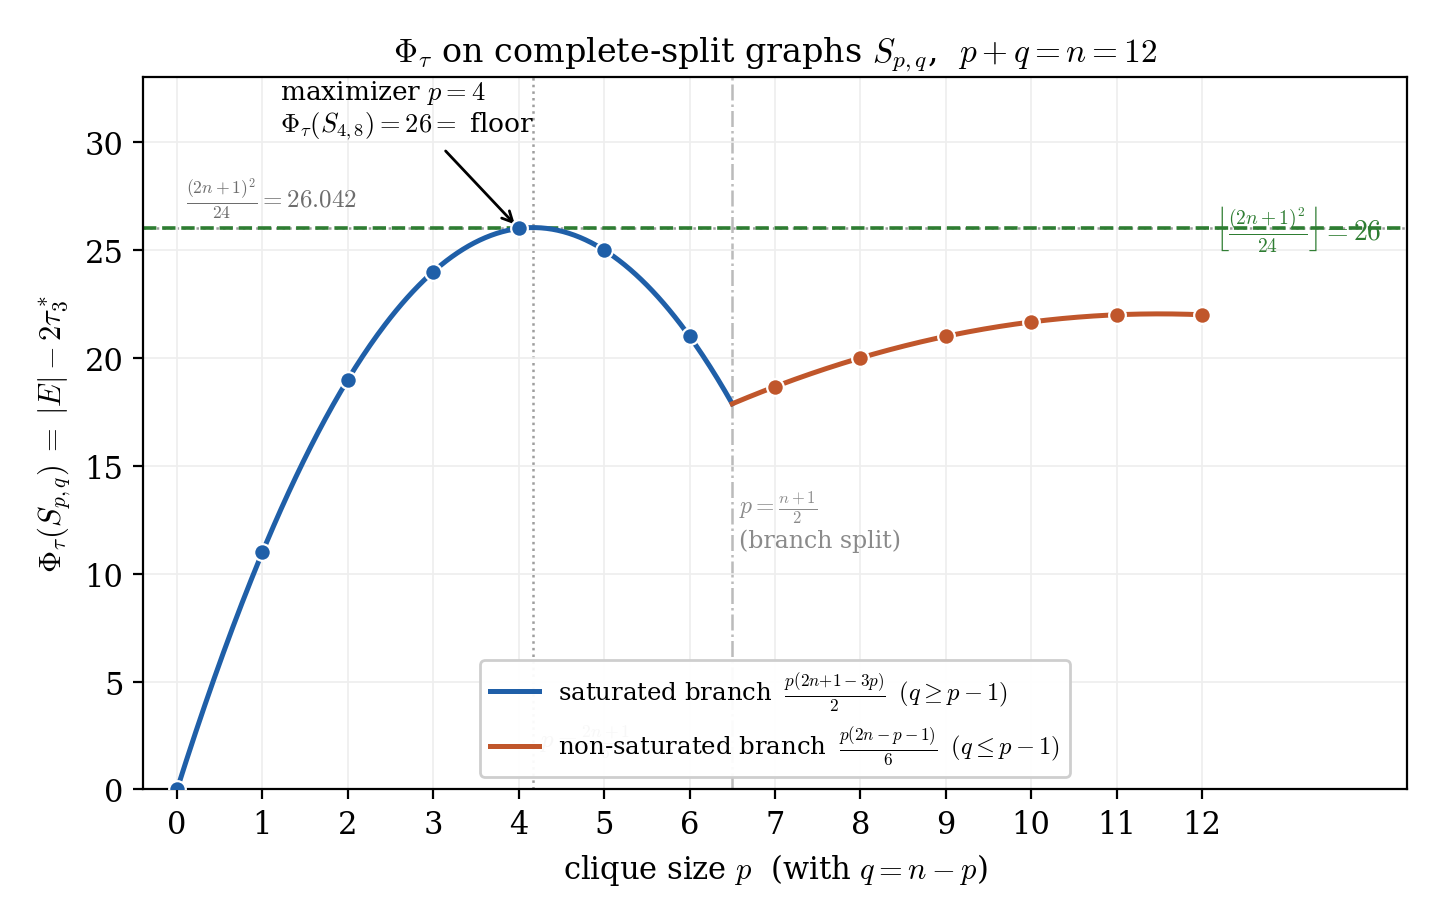
\includegraphics[width=0.8\textwidth,height=\textheight]{figures/fig2_phitau_profile.png}
\caption{Perfil de \(\Phi_\tau(S_{p,q})\) sobre grafos complete-split
con \(p+q=12\). La rama azul es el caso saturado \(q\ge p-1\), con valor
\(p(2n+1-3p)/2\); la rama naranja es el caso no saturado \(q\le p-1\),
con valor \(p(2n-p-1)/6\). El máximo entero se alcanza en \(p=4\), y es
\(\left\lfloor(2n+1)^2/24\right\rfloor=26\).}
\end{figure}

Los casos \(n=1,2\) coinciden con la misma fórmula. Para \(n=1\), el
único grafo tiene valor \(0\), y \(\lfloor9/24\rfloor=0\). Para \(n=2\),
el máximo es \(1\), alcanzado por \(K_2=S_{2,0}\), y
\(\lfloor25/24\rfloor=1\).

\begin{center}\rule{0.5\linewidth}{0.5pt}\end{center}

\section{8. Reproducibilidad, verificación formal y
alcance}\label{reproducibilidad-verificaciuxf3n-formal-y-alcance}

La prueba del artículo es analítica. Durante el desarrollo se usaron
experimentos computacionales para buscar contraejemplos y detectar
errores de transcripción, pero ningún cálculo computacional se usa como
premisa de la prueba.

El ledger de cálculo acompañante registra la prueba con un nivel más
bajo de granularidad. Lista las definiciones, la construcción de la
cobertura copiada en el Lema 3.1, las dos identidades de cancelación, la
elevación por convexidad discreta a clases de clones, el argumento de
progreso de clones, el requisito de simplicialidad en la reducción
cordal, la caracterización terminal complete-split, el programa de dos
variables en \(S_{p,q}\), el caso degenerado \(S_{2,0}\), las fórmulas
para \(\Phi_\tau(S_{p,q})\), y la maximización entera final. El teorema,
la cota exacta y el ensamblaje han recibido auditoría adversarial
interna. Esto es un registro del proceso de validación del autor, no una
afirmación de revisión externa por pares.

\subsection{Verificación formal en
Lean}\label{verificaciuxf3n-formal-en-lean}

El Teorema 1.1 está verificado formalmente en Lean 4 con Mathlib v4.28.0
{[}5,6{]}. La declaración correspondiente es

\[
\texttt{PaperII.theorem\_1\_2}
\]

en el repositorio {[}7{]}, commit \texttt{5f2d448}. El teorema formal
incluye ambos lados del resultado: la cota superior sobre todos los
grafos cordales con \(n\) vértices y la existencia de un grafo
complete-split que alcanza el valor.

La formalización usa el predicado cordal estándar \texttt{IsChordal}. En
el desarrollo, este predicado dice que todo ciclo de longitud al menos
cuatro tiene una cuerda. El funcional de déficit se formaliza como

\[
\texttt{phiTau G = (|E(G)| : ℝ) - 2 · tau3star G},
\]

donde \texttt{tau3star} es el número fraccional de cobertura de
triángulos del LP finito de cobertura. La familia complete-split se
formaliza como \texttt{completeSplit\ p\ q}, y el valor extremal es el
entero \(\lfloor(2n+1)^2/24\rfloor\).

No se agrega ningún axioma de estructura cordal. La formalización deriva
de \texttt{IsChordal} la propiedad hereditaria para subgrafos inducidos,
la preservación al agregar un vértice con vecindario clique, y la
existencia de vértices simpliciales. La prueba escrita del Lema 5.1 usa
árboles de cliques como infraestructura estándar de libro; la prueba
Lean usa un argumento de caracterización terminal sin árboles de
cliques. Por lo tanto, la prueba formal no asume un axioma de árbol de
cliques ni de intersección por caminos.

El desarrollo verificado cubre la desigualdad de cobertura copiada, la
convexidad discreta para clases de clones, el progreso de clases de
clones, la copia que preserva cordalidad, la caracterización terminal
complete-split, el promedio por órbitas en \(S_{p,q}\), el programa
lineal terminal y la maximización entera exacta. La compilación termina
exitosamente y no contiene \texttt{sorry}. El reporte de axiomas
registrado es

\begin{Shaded}
\begin{Highlighting}[]
\NormalTok{\#print axioms PaperII.theorem\_1\_2}
\NormalTok{[propext, Classical.choice, Quot.sound]}
\end{Highlighting}
\end{Shaded}

Estos son los axiomas clásicos estándar de Lean. El reporte no contiene
\texttt{sorryAx} ni axiomas específicos del proyecto. El certificado es
reproducible independientemente: se puede revisar el repositorio {[}7{]}
en el commit \texttt{5f2d448}, ejecutar \texttt{lake\ build}, y evaluar
\texttt{\#print\ axioms\ PaperII.theorem\_1\_2}.

\subsection{Verificación computacional
independiente}\label{verificaciuxf3n-computacional-independiente}

Además de la prueba analítica y del desarrollo Lean, scripts
independientes recomputaron las afirmaciones principales desde primeros
principios. Estos scripts evaluaron \(\tau_3^*\) mediante programación
lineal exacta, revisaron por separado el LP dual de empaquetamiento
fraccional como prueba de consistencia, realizaron la optimización
entera en aritmética racional exacta y usaron enumeración exhaustiva
cuando era factible. No se encontró ninguna discrepancia.

Las verificaciones incluyen:

\begin{itemize}
\tightlist
\item
  la desigualdad de copia de vértices y sus dos identidades de
  cancelación sobre todos los grafos no isomorfos con hasta \(7\)
  vértices y todos los pares no adyacentes;
\item
  convexidad discreta, progreso de clases de clones sin partición, y
  preservación de cordalidad, incluido un test con \(C_4\) que muestra
  por qué la hipótesis de simplicialidad es necesaria;
\item
  la caracterización terminal sobre todos los grafos cordales con hasta
  \(7\) vértices;
\item
  las fórmulas complete-split de la Proposición 6.2 y el Corolario 6.3
  contra el LP completo en el rango probado;
\item
  la identidad
  \(\max_{p+q=n}\Phi_\tau(S_{p,q})=\lfloor(2n+1)^2/24\rfloor\) para
  \(1\le n\le2000\);
\item
  el máximo global sobre grafos cordales, exhaustivamente para
  \(n\le7\), con pruebas aleatorias adicionales para \(8\le n\le12\).
\end{itemize}

Los scripts de auditoría, reportes y manifiestos SHA-256 acompañan el
preprint. Corroboran la prueba y ayudan a hacer reproducible el
lanzamiento; no sustituyen la prueba.

\subsection{Alcance}\label{alcance}

El resultado probado aquí es el extremo finito exacto del funcional
fraccional \(\Phi_\tau\). No es un teorema de particiones en cliques y
no usa empaquetamiento integral de triángulos. Dentro del programa del
Problema \#81 de Erdős, el rol de este artículo es identificar la
familia terminal complete-split y el valor fraccional exacto.

\begin{center}\rule{0.5\linewidth}{0.5pt}\end{center}

\section{Agradecimientos}\label{agradecimientos}

El autor agradece profundamente a su esposa María Paz y a sus hijos
Lucas, Juan Cristóbal, Francisca, Raimundo y Benjamín por su amor,
paciencia y apoyo.

\begin{center}\rule{0.5\linewidth}{0.5pt}\end{center}

\section{Uso de herramientas asistidas por
IA}\label{uso-de-herramientas-asistidas-por-ia}

Se usaron herramientas asistidas por IA durante las etapas
exploratorias, computacionales, adversariales, organizacionales y
editoriales, incluidos sistemas de Anthropic, Google y OpenAI. Estas
herramientas apoyaron la prueba de argumentos candidatos, chequeos
exactos de regresión, organización de pruebas, preparación de auditorías
y redacción. El autor revisó el contenido matemático, seleccionó los
argumentos finales y es el único responsable de las afirmaciones, citas,
código y presentación. Ningún sistema de IA figu